\documentclass[11pt,a4paper]{article}

% ---------------------------------------------------------------------------
% Reliable covalent export from an autocatalytic reactor under driven
% cleavage: explicit finite-copy operating, output and supply certificates.
%
% Author metadata: set the three macros below before submission.
% They are deliberately left blank in this version.
% ---------------------------------------------------------------------------
\newcommand{\PaperAuthor}{}
\newcommand{\PaperAffiliation}{}
\newcommand{\PaperDate}{14 September 2026}
% Author of the companion manuscript in refs.bib; replace by the author list.
\newcommand{\CompanionAuthor}{Anonymous}

\usepackage[T1]{fontenc}
\usepackage[utf8]{inputenc}
\usepackage{lmodern}
\usepackage{microtype}
\usepackage[a4paper,margin=1.05in]{geometry}
\usepackage{amsmath,amssymb,amsthm,mathtools}
\usepackage{booktabs}
\usepackage{array}
\usepackage{enumitem}
\usepackage{xcolor}
\usepackage{graphicx}
\usepackage{tikz}
\usetikzlibrary{arrows.meta,positioning,calc,decorations.pathreplacing}
\usepackage[obeyspaces,spaces]{url}
\usepackage[numbers,sort&compress]{natbib}
\usepackage[colorlinks=true,linkcolor=blue!55!black,citecolor=blue!55!black,urlcolor=blue!55!black]{hyperref}
\hypersetup{pdftitle={Reliable covalent export from an autocatalytic reactor under driven cleavage},
  pdfkeywords={autocatalysis, template replication, stochastic reaction networks, Foster-Lyapunov, uniformization, chemostat, chemical work, origin of life, Lean}}

\DeclareUrlCommand\lean{\urlstyle{tt}}
\setlist{itemsep=2pt,topsep=3pt}
\setlength{\emergencystretch}{1.5em}
\graphicspath{{figures/}}

\theoremstyle{plain}
\newtheorem{theorem}{Theorem}[section]
\newtheorem{proposition}[theorem]{Proposition}
\newtheorem{lemma}[theorem]{Lemma}
\newtheorem{corollary}[theorem]{Corollary}
\theoremstyle{definition}
\newtheorem{definition}[theorem]{Definition}
\theoremstyle{remark}
\newtheorem{remark}[theorem]{Remark}

\newcommand{\E}{\mathbb E}
\newcommand{\Prob}{\mathbb P}
\newcommand{\N}{\mathbb N}
\newcommand{\G}{\mathcal G}
\newcommand{\R}{\mathcal R_V}
\newcommand{\ind}{\mathbf 1}
\newcommand{\eps}{\varepsilon}
\newcommand{\cE}{c_{\mathrm E}}
\newcommand{\cW}{c_{\mathrm W}}
\newcommand{\BE}{B_{\mathrm E}}
\newcommand{\BR}{B_{\mathrm R}}
\newcommand{\BY}{B_{\mathrm Y}}
\newcommand{\BS}{B_{\mathrm S}}
\newcommand{\Son}{\mathcal S}
\newcommand{\Ooff}{\mathcal O}
\newcommand{\Ewin}{E_{\mathrm{win}}}
\newcommand{\Poff}{\Prob_{\mathrm{off}}}

\title{Reliable covalent export from an autocatalytic reactor\\ under driven cleavage:\\[4pt]
\large explicit finite-copy operating, output and supply certificates over an exponential horizon}
\author{\PaperAuthor\\ \small \PaperAffiliation}
\date{\PaperDate}

\begin{document}
\maketitle

\begin{abstract}
We prove an explicit reliability theorem for a six-species continuous-flow autocatalytic reactor with reversible substrate binding, templated ligation, duplex release, and an additional maintained-drive cleavage pathway that returns free covalent product to its two food components. The model is the literal integer-count Markov jump process with mass-action propensities, twenty labelled channels, and a copy scale $V$. Starting from food alone, the reactor establishes a catalytic population by a fixed deadline and then exports a prescribed amount of covalent product in every completed unit observation window. Uniformly over a fixed positive cleavage interval $\delta\in[1/100,1/20]$ and the kinetic box $K\in[8,12]$, $r\in[18,22]$, the joint operating event through time $500+e^{V/10^6}$ has probability at least $1-2e^{-2\times10^{-8}V}$ for every integer $V\ge10^8$. The event includes resource retention, post-entry residence, output in each of $\lfloor e^{V/10^6}\rfloor$ windows, and separate gross budgets for food input and for the driving service. A directly proved finite-duration version lets a reader choose any post-startup duration $H\ge1$ and obtain a certificate whose supply allowances are proportional to $500+H$; a sufficient copy scale follows from $H$ and a target failure probability. Removing only the templated ligation pair makes the same output schedule exponentially unlikely under a comparison that credits every resource exit as a possible success. Deterministic consequences give output on arbitrarily aligned intervals, expected export, resident inventory of order $V$ against replenishment of order $VT$, and explicit service and recovery ratios. The proof is a chain of generator inequalities on finite stopped uniformized kernels: startup is paid once, one-window output is bounded pointwise in the chemical state and propagated through the actual continuing distribution, and shared failures are charged once outside the window sum, so no independence between windows is assumed. The finite-kernel probability statements are verified in Lean~4 with Mathlib; nonexplosion of the infinite-state process and its identification with the finite construction are proved conventionally. A worked dimensional example illustrates the bounds without asserting experimental calibration.
\end{abstract}

\section{Introduction}\label{sec:intro}

Structural theories of autocatalysis, from Kauffman's autocatalytic sets~\citep{kauffman1986} and the RAF formalism of Hordijk and Steel~\citep{hordijk2004,steel2019} to the stoichiometric classification of autocatalytic cores~\citep{blokhuis2020}, certify that a reaction network can in principle make its own catalysts from a food source. Experimental template replicators~\citep{vonkiedrowski1986,sievers1994,lincoln2009} and kinetic design principles for minimal templated autocatalysts~\citep{sakref2024} show what such mechanisms look like chemically. Neither kind of result answers the operational question that a small open reactor actually poses: starting with no catalyst at all, does the reactor establish catalytic material, keep enough of it against washout, reversible sequestration~\citep{szathmary1989} and active destruction, and deliver product outside the reactor, repeatedly, for a long time, and at what supply cost?

A companion manuscript~\citep{predecessor2026} answered a fixed-horizon version of this question for one explicit six-species reactor at copy scale $V=10^8$: with probability at least $9/10$ the reactor establishes catalysis by time $500$ and exports at least $10^7$ covalent mass units during $(500,1000]$, and deleting only the templated ligation pair makes a conservative version of the same export event exponentially unlikely. Three things were left open there. The result was stated at one copy scale and one window. The reactor contained no active destruction pathway, so the certificate said nothing about tolerance to a competing loss. And the supply side of the ledger was implicit: a reactor that runs for a long time is continuously fed, and any claim about operation over a long horizon should say how much food and how much external driving the guaranteed operation may consume.

This paper closes all three. We add to the reactor a maintained-drive cleavage pair $X+F\rightleftharpoons U+W+P$, in which an externally maintained fuel $F$ returns free covalent product $X$ to its two food components while producing a maintained waste $P$, with a positive reverse rate. The competitor has fixed positive strength $\delta\in[1/100,1/20]$ that does not shrink with the copy scale. We then prove, uniformly over the kinetic box and for every integer copy scale $V\ge10^8$, that the reactor establishes catalysis by time $500$ and exports at least $V/5000$ covalent mass units in every one of $\lfloor e^{V/10^6}\rfloor$ consecutive unit windows, while resources stay in a corridor, the catalytic population stays above a floor, each food input count stays below $2V\cdot(500+e^{V/10^6})$, and the gross number of driving events stays below one eighth of $V$ times the elapsed time; the joint probability is at least $1-2e^{-2\times10^{-8}V}$. A finite-duration form of the same theorem (Theorem~\ref{thm:main}) gives, for any chosen post-startup duration $H\ge1$, an explicit error budget whose supply allowances scale with $500+H$ rather than with the exponential horizon. Since the copy scale is a free integer, the certificate is a design rule: a target duration and a target confidence determine a sufficient $V$ (Section~\ref{sec:example}).

\paragraph{Method.}
All estimates are Foster--Lyapunov generator inequalities~\citep{meyn1993} used quantitatively over a finite horizon on finite stopped models through uniformization~\citep{jensen1953,grassmann1977}. In the stochastic reaction network literature such inequalities usually serve long-time properties such as positive recurrence and moment bounds~\citep{gupta2014,anderson2018}; here every bound is a number obtained from an explicit drift constant and a kernel $P=I+\G/q$. Five ingredients are specific to the long horizon and the competitor. First, the added channels conserve both resource moieties, so the resource-restoration estimate of the fixed-horizon result survives unchanged. Second, the cleavage loss acts on free product only, whereas the tight phase of the weighted catalytic count is a bound complex; exploiting that slack channel by channel keeps the low-count growth and noise constants unchanged on the whole cleavage interval, so the changing-exponential startup schedule can be reused. Third, the entry threshold and residence floor scale with $V$, which turns a fixed return barrier into a volume exponent. Fourth, one-window output is bounded pointwise in the chemical state by a marked-export tilt with a saturating counter; the bound is propagated through the actual continuing chemical distribution by induction over windows, with a persistent history bit, so that $m$ windows cost $m$ times one bound while entry, resource and return failures are charged once. Fifth, four gross supply counters ride along the same law, and their exponential moments compose through startup, every window boundary and the final fraction; saturation lemmas show that a capped counter cannot hide a budget violation. The final inequality is a union bound on one law.

\paragraph{Formal verification.}
The finite-kernel statements, including all numerical constants and the induction over windows, have been checked in Lean~4~\citep{demoura2021} with Mathlib~\citep{mathlib2020}. Appendix~\ref{app:formal} lists the declarations and the reproduction command. The identification of the finite stopped construction with the literal infinite-state reaction process, including nonexplosion, is a conventional argument written out in Section~\ref{sec:formal}; the paper states at each point which side of this boundary a statement lies on.

\paragraph{What is not claimed.}
The theorem is a statement about one explicit mechanism and parameter box. It does not give an optimal cleavage tolerance, an optimal lifetime exponent, or a large-deviation rate function; the general theory of~\citep{agazzi2018} would be the route to such asymptotics, and our explicit constants are not sharp. Exponential finite horizons are not perpetual survival: the count process is positive recurrent at fixed $V$, so catalyst loss eventually occurs, and only finite-time operation is the correct object. No experimental rate has been fitted, the two reservoirs are modelled as maintained activities in the sense of open-network thermodynamics~\citep{polettini2014,rao2016,rao2018}, and the dimensional example in Section~\ref{sec:example} is a translation of units, not a calibrated protocol. Nothing is asserted about sliding windows, arbitrary initial states or stationary productivity.

\paragraph{Organisation.}
Section~\ref{sec:model} specifies the reactor and the observables. Section~\ref{sec:theorem} defines the operating event and states the main theorem. Section~\ref{sec:formal} gives the finite stopped construction and the conventional identification. Section~\ref{sec:proof} proves the theorem, Section~\ref{sec:disabled} the disabled comparison, Section~\ref{sec:consequences} the deterministic consequences, Section~\ref{sec:example} the sizing rule, worked example and reservoir-work interpretation. Section~\ref{sec:discussion} discusses scope. The appendices record the coefficient checks, the elementary inequalities and the formal evidence.

\section{The reactor}\label{sec:model}

\subsection{Species, channels and parameters}

The count state is $n=(u,w,x,c_1,c_2,z)\in\N^6$. Foods $U,W$ are supplied from outside. Their covalent ligation gives the product $X=UW$, which is also the template. A template binds its substrates in two steps, $X+U\rightleftharpoons C_1=X{:}U$ and $C_1+W\rightleftharpoons C_2=X{:}(U,W)$; ligation inside $C_2$ gives a duplex $Z=X{:}X$, which releases two free templates. Fix
\begin{equation}\label{eq:box}
 V\in\N,\quad V\ge10^8,\qquad
 \eps=\frac1{500\,000\,000},\qquad
 K\in[8,12],\qquad r\in[18,22],\qquad
 \delta\in\Big[\frac1{100},\frac1{20}\Big],
\end{equation}
and write $k=K^{-1}$ and $\eta=\eps/16$. The initial state is $n_0=(V,V,0,0,0,0)$. Time is dimensionless with dilution coefficient one. Table~\ref{tab:source} lists the twenty labelled channels with their count propensities and observation marks, and Figure~\ref{fig:scheme} shows the mechanism. The eighteen channels $0$--$17$ are those of the companion reactor~\citep{predecessor2026}. The added pair is
\begin{equation}\label{eq:drive}
 X+F\ \mathop{\rightleftharpoons}^{\ \delta x\ }_{\delta\eta\,uw/V}\ U+W+P,
\end{equation}
where $F$ and $P$ are externally maintained reservoirs whose fixed activities have been absorbed into the coefficients; they are not dynamical species. In the six count coordinates the pair changes the state exactly as basal cleavage and basal ligation (channels $1$ and $0$), but with a different ratio and with distinct service labels. The templated reverse coefficient of channel $7$ remains $20k$.

\begin{table}[t]
\centering\small
\caption{The twenty-channel source. A mark is the increment of the indicated cumulative counter; food and driving marks are ordered pairs. Every unlisted mark is zero. The association propensity in channel $9$ is the falling factorial $rx(x-1)/V$ with no additional factorial divisor. Channels $6$ and $7$ are the only channels removed in the disabled comparison of Section~\ref{sec:disabled}.}\label{tab:source}
\begin{tabular}{rllccc}
\toprule
$j$ & Reaction & Count propensity & Export $e_j$ & $(I_U,I_W)$ & $(Q_F,Q_P)$\\
\midrule
0 & $U+W\to X$ & $\eps uw/V$ & 0 & $(0,0)$ & $(0,0)$\\
1 & $X\to U+W$ & $\eps kx$ & 0 & $(0,0)$ & $(0,0)$\\
2 & $X+U\to C_1$ & $20xu/V$ & 0 & $(0,0)$ & $(0,0)$\\
3 & $C_1\to X+U$ & $20c_1$ & 0 & $(0,0)$ & $(0,0)$\\
4 & $C_1+W\to C_2$ & $20c_1w/V$ & 0 & $(0,0)$ & $(0,0)$\\
5 & $C_2\to C_1+W$ & $20c_2$ & 0 & $(0,0)$ & $(0,0)$\\
6 & $C_2\to Z$ & $20c_2$ & 0 & $(0,0)$ & $(0,0)$\\
7 & $Z\to C_2$ & $20kz$ & 0 & $(0,0)$ & $(0,0)$\\
8 & $Z\to2X$ & $rz$ & 0 & $(0,0)$ & $(0,0)$\\
9 & $2X\to Z$ & $rx(x-1)/V$ & 0 & $(0,0)$ & $(0,0)$\\
\midrule
10 & $\varnothing\to U$ & $V$ & 0 & $(1,0)$ & $(0,0)$\\
11 & $\varnothing\to W$ & $V$ & 0 & $(0,1)$ & $(0,0)$\\
12 & $U\to\varnothing$ & $u$ & 0 & $(0,0)$ & $(0,0)$\\
13 & $W\to\varnothing$ & $w$ & 0 & $(0,0)$ & $(0,0)$\\
14 & $X\to\varnothing$ & $x$ & 4 & $(0,0)$ & $(0,0)$\\
15 & $C_1\to\varnothing$ & $c_1$ & 4 & $(0,0)$ & $(0,0)$\\
16 & $C_2\to\varnothing$ & $c_2$ & 4 & $(0,0)$ & $(0,0)$\\
17 & $Z\to\varnothing$ & $z$ & 8 & $(0,0)$ & $(0,0)$\\
\midrule
18 & $X+F\to U+W+P$ & $\delta x$ & 0 & $(0,0)$ & $(1,0)$\\
19 & $U+W+P\to X+F$ & $\delta\eta uw/V$ & 0 & $(0,0)$ & $(0,1)$\\
\bottomrule
\end{tabular}
\end{table}

\begin{figure}[t]
\centering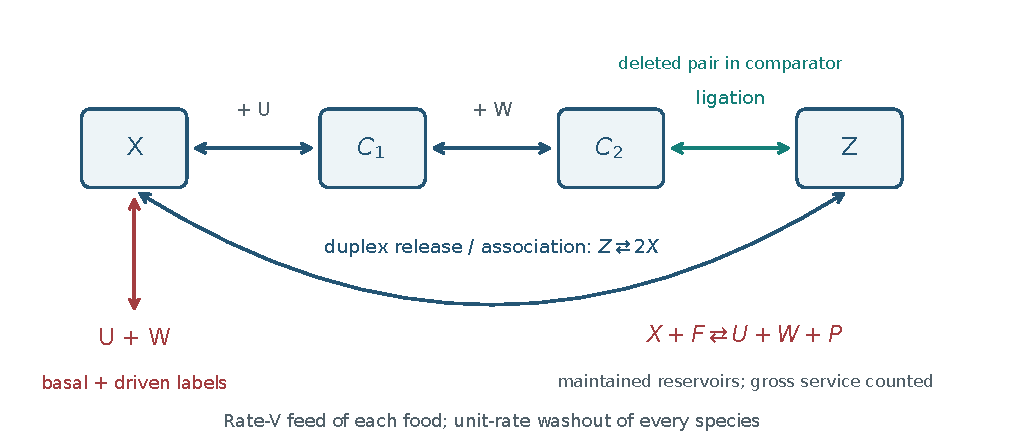
\includegraphics[width=0.92\linewidth]{reaction_scheme.pdf}
\caption{Internal pathway and maintained driving service. All displayed internal arrows are reversible; the complete rates and marks are in Table~\ref{tab:source}. The pair deleted in the comparator is only $C_2\rightleftharpoons Z$. Food feed and washout continue in both systems.}\label{fig:scheme}
\end{figure}

The generator is $\G f(n)=\sum_{j=0}^{19}a_j(n)[f(n+\nu_j)-f(n)]$, where $\nu_j$ subtracts the reactants and adds the products of channel $j$. Every positive-rate channel has its reactants available, so the process never leaves $\N^6$. The number $V$ is a copy scale: it divides every bimolecular propensity and equals each feed rate, so that concentrations $n/V$ obey the classical density-dependent scaling~\citep{kurtz1972,anderson2015}. The parameter $K$ is the equilibrium bias of the two ligation steps, and $r$ sets the time scale of duplex release relative to binding and unbinding, whose coefficient is $20$.

\begin{remark}[Reservoir consistency]\label{rem:affinity}
The basal pair (channels $0,1$) has effective ratio $x/(uw)=K$ at internal equilibrium, whereas the driven pair (channels $18,19$) has ratio $\eta=\eps/16$. They cannot both be undriven detailed-balanced pairs of the same internal equilibrium. With standard potentials chosen consistently with the five reversible internal pairs, the two reservoirs must maintain the affinity
\begin{equation}\label{eq:affinity}
 \frac{\mu_F-\mu_P}{k_BT_{\mathrm{phys}}}=\log\frac K\eta=\log(8\times10^9K),
\end{equation}
which is $24.882$--$25.288$ across the box, or $61.65$--$62.66$ kJ/mol at $298$~K. Basal ligation followed by driven cleavage is then a cycle with this nonzero affinity: the reactor is chemostatted in the sense of~\citep{polettini2014,rao2016}. Equation~\eqref{eq:affinity} is a thermodynamic requirement of this illustrative model, not an identification of a particular fuel.
\end{remark}

\subsection{Observables}

Define the two resource moieties, the weighted catalytic count, the resident mass and the covalent stock by
\begin{align}
 A&=u+x+2c_1+2c_2+2z,& B&=w+x+c_1+2c_2+2z,\label{eq:AB}\\
 Y&=x+\tfrac98c_1+\tfrac75c_2+\tfrac95z,\label{eq:Y}\\
 M&=2(A+B)=2u+2w+4x+6c_1+8c_2+8z,\label{eq:M}\\
 S&=4x+4c_1+4c_2+8z.\label{eq:S}
\end{align}
Every internal channel, including the driven pair, preserves $A$ and $B$; only feeds and washouts change them. The corridor is $\R=\{0.9V\le A,B\le1.1V\}$. Let $E(t)$ be the uncapped cumulative export with the marks $e_j$ of Table~\ref{tab:source}, so that $E/4$ counts covalent $X$ equivalents leaving the reactor in free product, in complexes and in duplexes. Bound food is not covalent product, and cleavage is not export. Let $I_U,I_W$ count the two feed channels, $Q_F,Q_P$ the two driving directions, and $Q_D=Q_F+Q_P$ their \emph{gross} sum; the difference $Q_F-Q_P$ is not used as a cost proxy. Let $\tau$ be the first time $Y\ge V/2500$ and $\sigma$ the first subsequent time $Y\le V/5000$. The weights in~\eqref{eq:Y} count bound complexes more than free product; the reason is visible in the drift expansion~\eqref{eq:driftexpansion} below.

\begin{remark}[Startup is an immigration problem]\label{rem:startup}
At $n_0$ every channel that needs $X,C_1,C_2$ or $Z$ has zero propensity. Catalytic material first appears through channels $0$ or $19$, with combined propensity $(\eps+\delta\eta)uw/V=b_+V$ at $n_0$, where $b_+=\eps+\delta\eta\le\eps(1+1/320)$. Before the first such event the foods are two independent immigration--death processes with rate $V$ and unit death rate, and $\E(\bar U_t\bar W_t)=V^2$. Conditioning on the food path and applying Jensen's inequality to the first-creation clock gives
\[
 \Prob(\text{no catalytic species by time }T)=\E\exp\Big[-\frac{b_+}V\int_0^T\bar U_t\bar W_t\,dt\Big]\ge e^{-b_+VT}.
\]
At $V=10^8$ and $\delta=1/20$ the probability of no seed by time $1$ is at least $0.818$, and any deadline with $90\%$ startup must exceed $\log(10)/(b_+V)\ge11.47$. The fixed deadline $500$ of the theorem is therefore not an artefact of the proof technique alone; this necessary condition is a conventional remark, not part of the formal development.
\end{remark}

\section{The operating event and the main theorem}\label{sec:theorem}

For any requested post-startup duration $H\ge1$ put
\begin{equation}\label{eq:duration}
 T_H=500+H,\qquad m_H=\lfloor H\rfloor,\qquad s_H=H-m_H\in[0,1).
\end{equation}
The observation schedule is shown in Figure~\ref{fig:timeline}.

\begin{definition}[Operating event]\label{def:event}
The event $\Son_H$ requires all of the following on one trajectory started at $n_0$:
\begin{enumerate}[label=(\roman*)]
\item \emph{startup and residence:} $\tau\le500$, $n(t)\in\R$ for all $0\le t\le T_H$, and $\sigma>T_H$;
\item \emph{repeated output:} $E(501+i)-E(500+i)\ge V/5000$ for every integer $0\le i<m_H$;
\item \emph{supplies:} $I_U(T_H)\le2VT_H$, $I_W(T_H)\le2VT_H$ and $Q_D(T_H)\le VT_H/8$.
\end{enumerate}
\end{definition}
The final fractional interval of length $s_H$ is subject to the residence, resource and supply conditions but adds no complete-window output condition.

\begin{figure}[t]
\centering
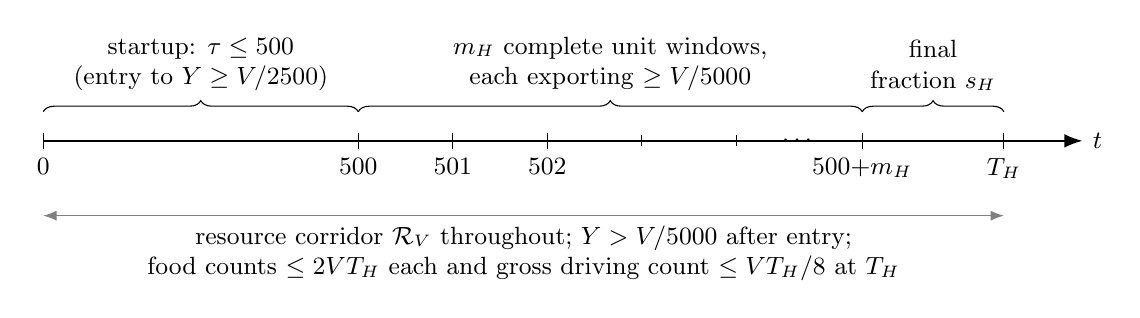
\begin{tikzpicture}[>=Latex,font=\small,x=1cm]
\draw[->,thick] (0,0) -- (13.2,0) node[right] {$t$};
\foreach \x/\l in {0/$0$,4/$500$,5.2/$501$,6.4/$502$,10.4/$500{+}m_H$,12.2/$T_H$} {\draw (\x,-0.1)--(\x,0.1); \node[below] at (\x,-0.1) {\l};}
\foreach \x in {7.6,8.8} {\draw (\x,-0.07)--(\x,0.07);}
\node at (9.6,0) {$\cdots$};
\draw[decorate,decoration={brace,amplitude=4pt,raise=2pt}] (0,0.3)--(4,0.3) node[midway,above=6pt,align=center] {startup: $\tau\le500$\\(entry to $Y\ge V/2500$)};
\draw[decorate,decoration={brace,amplitude=4pt,raise=2pt}] (4,0.3)--(10.4,0.3) node[midway,above=6pt,align=center] {$m_H$ complete unit windows,\\each exporting $\ge V/5000$};
\draw[decorate,decoration={brace,amplitude=4pt,raise=2pt}] (10.4,0.3)--(12.2,0.3) node[midway,above=6pt,align=center] {final\\fraction $s_H$};
\draw[<->,gray] (0,-0.95)--(12.2,-0.95) node[midway,below,black,align=center] {resource corridor $\R$ throughout; $Y>V/5000$ after entry;\\food counts $\le2VT_H$ each and gross driving count $\le VT_H/8$ at $T_H$};
\end{tikzpicture}
\caption{The observation schedule of Definition~\ref{def:event}. Windows begin at deterministic times; only the measurement counter is reset at a window boundary, the chemical state and all cumulative supply counters persist.}\label{fig:timeline}
\end{figure}

Define the constants and error terms
\begin{align}
 \cE&=\frac{8047}{312\,500\,000\,000}\approx2.575\times10^{-8},&
 \cW&=\frac{13}{1\,080\,000}\approx1.204\times10^{-5},\label{eq:constants}\\
 \BE(V)&=e^{-\cE V}+e^{-3V/500},\label{eq:entryB}\\
 \BR(V,T)&=4e^{-V/1000}+12000\,VT\,e^{1/50-V/2000},\label{eq:resB}\\
 \BY(V,T)&=e^{-V/62500}+3000\,VT\,e^{18/125-V/15625},\label{eq:retB}\\
 \BS(V,T)&=2e^{-(2\log2-1)VT}+e^{-VT/200},\label{eq:supB}\\
 \mathcal B(V,H)&=\BE(V)+\BR(V,T_H)+\BY(V,T_H)\notag\\
 &\qquad+m_He^{1/8-\cW V}+\BS(V,T_H).\label{eq:budget}
\end{align}
Each term is the price of one failure mode: missed entry and the startup clock, resource exit, post-entry return, an insufficient window, and the three supply budgets.

\begin{theorem}[Joint operation, repeated output and supplies]\label{thm:main}
Under~\eqref{eq:box}, for every $H\ge1$,
\begin{equation}\label{eq:finite}
 \Prob(\Son_H)\ge\max\{0,\,1-\mathcal B(V,H)\}.
\end{equation}
In particular, for the exponential horizon
\begin{equation}\label{eq:exphorizon}
 D=e^{V/10^6},\qquad T=500+D,\qquad m=\lfloor D\rfloor,
\end{equation}
one has
\begin{equation}\label{eq:main}
 \Prob(\Son_D)\ge1-2e^{-bV},\qquad b=2\times10^{-8},
\end{equation}
and the same simplified bound holds for $\Son_H$ whenever $1\le H\le D$, with the duration-specific supply budgets $2VT_H$ and $VT_H/8$.
\end{theorem}

Three comments on the statement. First, the constants in~\eqref{eq:main} are a uniform simplification and are far from sharp at $V=10^8$: there the full budget~\eqref{eq:budget} gives $\Prob(\Son_{100})\ge0.9238$ while~\eqref{eq:main} gives only $0.7293$ (Section~\ref{sec:example}). Second, the last assertion is not a restriction of $\Son_D$: restricting the exponential-horizon event would keep its astronomical supply allowances, whereas the finite-duration allowances are proportional to $T_H$ and are proved directly (Lemma~\ref{lem:supplies}). Third, the finite marked-kernel counterparts of~\eqref{eq:finite} and~\eqref{eq:main} are the Lean exports of Appendix~\ref{app:formal}; the passage to the literal infinite-state process is the conventional construction of the next section, and that boundary is part of the evidence statement of the theorem.

\section{The finite stopped law and the common process}\label{sec:formal}

\paragraph{Nonexplosion.}
Internal channels conserve $A+B$, and the only increases of $A+B$ are the two rate-$V$ feed channels. Hence pathwise, on every finite interval,
\begin{equation}\label{eq:nonexplosion}
 A(t)+B(t)\le2V+I_U(t)+I_W(t).
\end{equation}
The feed counts can be generated by two independent rate-$V$ Poisson clocks, which are finite almost surely on compact time intervals and bound all six species there. Each bounded set of counts is finite and carries finite total rates, so localization at successive resource levels rules out infinitely many jumps in finite time. The minimal process is therefore nonexplosive~\citep{anderson2015}; the same argument applies after removing channels $6$ and $7$.

\paragraph{Finite stopped construction.}
On $\R$ every coordinate is at most $1.1V$. Embed the counts in a finite box strictly larger than this corridor, retain the first state outside the corridor, and set all rates to zero after a declared resource or return failure. The box update equals the exact stoichiometric update for every transition from a corridor state, including the first exiting transition, so no transition of interest is clipped. Direct source bounds give the uniform rate cap
\begin{equation}\label{eq:clock}
 \sum_ja_j(n)\le q_V:=3000V
\end{equation}
on all active states; each inherited channel is at most $27V$ on the corridor, feeds contribute $2V$, washouts at most $6.6V$, and the two added channels together at most $\frac1{20}(1.1+1.21\eta)V<0.056V$, so the cap has ample slack. Uniformization~\citep{jensen1953,grassmann1977} gives the kernel $P=I+\G/q_V$, with transition probabilities $a_j/q_V$ and a self-loop that carries no reaction marks; a rate-$q_V$ Poisson clock realizes the finite stopped process, and every expectation below is a Poisson mixture of kernel powers.

The state carries, besides the counts, an entry/return phase, the current-window export counter, a persistent all-window pass bit, and the four cumulative supply counters. Entry missed at time $500$ is declared failure. At each window boundary $500+i$ only the measurement counter is reset; the chemical state, phase, pass bit and supply counters persist. A counter capped at $C$ records $\min\{C,\text{natural count}\}$; caps strictly above the relevant thresholds preserve every threshold violation, including violations of the sum $Q_F+Q_P$ (Lemma~\ref{lem:supplies}). Reaching the export cap in a window never stops the chemistry.

\paragraph{One law.}
Forgetting the supply counters intertwines the actual kernels with the chemical/measurement kernels: the identity $\widetilde\G(f\circ\pi)=(\G f)\circ\pi$ for the projection $\pi$ transfers to kernel powers by induction, to Poisson mixtures by summation, and to the startup/window/final-fraction composition. Hence all failure events, chemical and supply, belong to one law, and a single union bound applies.

\paragraph{Identification.}
Couple the finite stopped construction to the literal reaction clocks until the first declared failure. Up to that time the two processes coincide, so artificial absorption affects only trajectories outside $\Son_H$, and the good event of the finite law is exactly $\Son_H$ for the literal process. This paragraph and the nonexplosion paragraph are conventional mathematics; the finite projections, saturation lemmas and probability bounds of the following sections are formally verified.

\section{Proof of the operating theorem}\label{sec:proof}

\subsection{Two generator inequalities}
For a uniformized finite kernel and a nonnegative test $F$, the elementary Foster and decay implications are
\begin{align}
 \G F\le L\ \ (F\ge0)&\quad\Longrightarrow\quad\E F(t)\le F(0)+Lt,\label{eq:foster}\\
 \G F\le-\kappa F\ \ (F\ge0)&\quad\Longrightarrow\quad\E F(t)\le e^{-\kappa t}F(0).\label{eq:decay}
\end{align}
Both follow by induction on kernel powers and summation against the Poisson law, and the second permits negative $\kappa$ when a growing exponential moment is bounded. Throughout we use the elementary inequality $e^v\le1+v+\frac35v^2$ for $|v|\le\frac9{50}$ (Appendix~\ref{app:ineq}).

\subsection{Resources}
\begin{lemma}[Resource restoration]\label{lem:resources}
Resource exit through time $T$ has probability at most $\BR(V,T)$, for the enabled and for the disabled source.
\end{lemma}
\begin{proof}
For $D_0\in\{A,B\}$, internal conservation and the feed/washout channels give
\[
 \G D_0=V-D_0,\qquad\sum_ja_j(\Delta_jD_0)^2\le V+2D_0,\qquad|\Delta_jD_0|\le2.
\]
For $|\theta|\le1/100$ the quadratic exponential inequality yields
$\sum_ja_j(e^{\theta\Delta_jD_0}-1)\le\theta(V-D_0)+\frac35\theta^2(V+2D_0)$.
Take the four tests $f^+_{D_0}=e^{(D_0-1.1V)/100}$ and $f^-_{D_0}=e^{-(D_0-0.9V)/100}$. Their tilted drifts are nonpositive when $D_0\ge1.05V$, respectively $D_0\le0.95V$. In the complementary region a destination potential is at most $e^{1/50-V/2000}$ because a moiety jump has size at most two, so dropping the negative current term bounds each generator by $q_Ve^{1/50-V/2000}$. The sum of the four tests equals $4e^{-V/1000}$ at $n_0$ and is at least one at the retained first exit state. Equation~\eqref{eq:foster} gives~\eqref{eq:resB}. Removing channels $6,7$ or adding channels $18,19$ leaves $\G D_0$ and the quadratic bound unchanged.
\end{proof}

\subsection{Low-count growth}
\begin{lemma}[Growth, noise and exponential control at low density]\label{lem:local}
On $\R\cap\{Y\le V/1000\}$, for every parameter in the box~\eqref{eq:box},
\begin{align}
 \G Y&\ge\frac{39}{100}Y+\frac{16}{25}\eps V,\label{eq:drift}\\
 Q_Y:=\sum_ja_j(\Delta_jY)^2&\le5Y+\frac{25}{16}\eps V,\qquad|\Delta_jY|\le\frac95,\label{eq:noise}\\
 \sum_ja_j\big(e^{-\theta\Delta_jY}-1\big)&\le-\Big(\frac3{10}\theta-3\theta^2\Big)Y-\frac{14}{25}\eps V\theta,\qquad0\le\theta\le\frac2{25}.\label{eq:tilt}
\end{align}
\end{lemma}
\begin{proof}
On the corridor with $Y\le V/1000$, free food satisfies $u,w\ge0.9V-2Y\ge\frac45V$ and $u,w\le1.1V$; also $x\le Y$. Exact count algebra over the twenty channels gives
\begin{equation}\label{eq:driftexpansion}
\begin{aligned}
 \G Y={}&(\eps+\delta\eta)\frac{uw}V-(\eps k+\delta)x+\Big(\frac{5u}{2V}-1\Big)x
 +\Big(-\frac{29}8+\frac{11w}{2V}\Big)c_1+\frac{11}{10}c_2\\
 &+\Big(\frac r5-\frac95-8k\Big)z-\frac r{5V}(x^2-x).
\end{aligned}
\end{equation}
The cleavage loss $-\delta x$ acts on free product only. The coefficient of $x$, after the basal term, the cleavage term and the quadratic term $-(r/5V)x^2\ge-(22/5000)x$, is at least $1-\frac1{20}-\frac{22}{5000}-\frac1{8\times10^6}>\frac{39}{100}$. The coefficients of $c_1,c_2,z$ are at least $\frac{31}{40},\frac{11}{10},\frac45$, which exceed $\frac{39}{100}$ times the weights $\frac98,\frac75,\frac95$. The falling-factorial correction $+rx/(5V)$ is nonnegative and the immigration term is at least $\frac{16}{25}\eps V$. This proves~\eqref{eq:drift}; the slack in the bound phases is what absorbs the competitor without changing the constant. (The same coefficient table holds for $0\le\delta\le3/5$, so the local estimate is not the binding constraint on the cleavage interval; the supply bounds and the disabled comparison were sized for the stated box.)

The signed $Y$-increments of the five internal pairs are $\pm1,\pm\frac18,\pm\frac{11}{40},\pm\frac25,\pm\frac15$; feeds and food washout have increment $0$, catalytic washout has the negative weight, and the driven pair has $\pm1$. Summing squares against propensities and using $x(x-1)\le x^2$ gives~\eqref{eq:noise}; the explicit envelope is in Appendix~\ref{app:coeff}. Finally the quadratic exponential inequality bounds the left side of~\eqref{eq:tilt} by $-\theta\G Y+\frac35\theta^2Q_Y$; substituting~\eqref{eq:drift}--\eqref{eq:noise} gives the $Y$-coefficient $-(\frac{39}{100}\theta-3\theta^2)\le-(\frac3{10}\theta-3\theta^2)$ and the immigration coefficient $\frac{16}{25}-\frac{15}{16}\cdot\frac2{25}=\frac{113}{200}>\frac{14}{25}$.
\end{proof}

\subsection{Startup and residence}
\begin{lemma}[Entry by the deadline; return after entry]\label{lem:entryreturn}
Missed entry without resource exit by time $500$ has probability at most $\BE(V)$. Return to $Y\le V/5000$ after entry, through time $T$, has probability at most $\BY(V,T)$.
\end{lemma}
\begin{proof}
\emph{Entry.} Use the auxiliary no-entry test
$F_\theta(n)=\ind_{\{n\in\R,\ Y<V/2500\}}e^{-\theta Y}$.
With $\alpha(\theta)=\frac3{10}\theta-3\theta^2$ and $\beta=\frac{14}{25}\eps V$, uniformization of~\eqref{eq:tilt} gives the transfer inequality
\begin{equation}\label{eq:transfer}
 PF_\theta\le e^{-\beta\theta/q_V}F_\zeta\qquad\text{whenever }0\le\theta\le\tfrac2{25}\text{ and }\zeta\le\theta+\alpha(\theta)/q_V,
\end{equation}
since killing the test after entry or resource exit only decreases its generator. The exponent therefore grows along the kernel steps while the indicator is converted at the initial exponent: $\ind_{\{\text{no entry}\}}\le e^{\theta_0V/2500}F_{\theta_0}$. Start at $\theta_0=1/40000$ and use the capped update $\theta\mapsto\min\{d,(1+c/q_V)\theta\}$, admissible when $c+3d\le\frac3{10}$: with $(c,d)=(\frac3{20},\frac1{20})$ for $90q_V$ steps and $(\frac3{50},\frac2{25})$ for $10q_V$ steps, Bernoulli's inequality on blocks of $10q_V$ steps gives growth factors at least $(5/2)^9>2000$ and $8/5$, so $\theta$ reaches $\frac2{25}$ within $100q_V$ steps. Dropping the decay factors during those steps and retaining them for the remaining $399q_V$ of $499q_V$ steps bounds the no-entry probability after $499q_V$ steps by
\[
 \exp\Big(\frac V{2500\cdot40000}-399\,\beta\,\frac2{25}\Big)=e^{-\cE V}.
\]
For the physical deadline, the number $J$ of kernel steps by time $500$ is Poisson$(500q_V)$, and the geometric test $(999/1000)^J$ gives $\Prob(J<499q_V)\le e^{-q_V/500000}=e^{-3V/500}$. Splitting the Poisson sum at $499q_V$ proves~\eqref{eq:entryB}. The auxiliary process agrees with the continuing process before entry or exit, and the no-entry test vanishes afterwards, so the bound applies to the actual law without choosing a post-entry composition.

\emph{Return.} Use the phase-dependent potential equal to the constant $e^{-V/62500}$ before entry and to $R(n)=e^{-(2/25)(Y-V/5000)}$ after entry. It does not increase at the entry jump (there $Y\ge V/2500$), and it is at least one at the first return. In the low-count region $Y\le V/1000$ inequality~\eqref{eq:tilt} with $\theta=\frac2{25}$ gives nonpositive drift. Above $Y=V/1000$ every destination has $Y'\ge V/1000-\frac95$, so its potential is at most $e^{18/125-V/15625}$, and the rate cap bounds the positive drift by $q_V$ times this. Equation~\eqref{eq:foster} from the initial state gives~\eqref{eq:retB}; the random entry state and its overshoot are paid once through the potential rather than by restarting at a chosen composition.
\end{proof}

\subsection{One window, and all windows}
\begin{lemma}[Marked export in one window; composition]\label{lem:windows}
After entry, resource and return failures are charged once, failure of any of the $m_H$ complete output windows contributes at most $m_He^{1/8-\cW V}$ to the error budget.
\end{lemma}
\begin{proof}
During residence $Y>V/5000$, the washout intensity of $X,C_1,C_2,Z$ is $x+c_1+c_2+z\ge\frac59Y>V/9000$, and every such washout exports at least four units. With the tilt $e^{-e_j/8}$ and $e^{-1/2}\le\frac23$,
\[
 \sum_ja_j\big(e^{-e_j/8}-1\big)\le-\frac5{27}Y\le-\frac V{27000}.
\]
Put $C=\lceil V/5000\rceil$ and use the killed test $\ind_{\{\text{active},\ c<C\}}e^{-c/8}$ on the current-window counter $c$. Its generator is at most $-V/27000$ times the test: a jump that reaches the cap sends the test to zero, and any other jump has the true export mark. Thus saturation preserves the inequality while chemistry continues. By~\eqref{eq:decay}, insufficient export after one unit of time has probability at most
\[
 e^{C/8-V/27000}\le e^{1/8-(13/1080000)V}=e^{1/8-\cW V},
\]
and this bound is pointwise in the chemical state at the start of the window. At a boundary the new pass indicator is conjoined with the persistent history bit and only $c$ is reset. A failed phase is absorbing; otherwise the probability that the history bit newly fails during the next window is at most the displayed bound, whatever the current chemical distribution. Induction over the actual successive kernels bounds the probability of any failed window by $m_H$ times the one-window bound, with no independence assumption. The resource and return Foster errors compose additively over the elapsed time, including $s_H$, rather than being restarted and multiplied by $m_H$.
\end{proof}

\subsection{Supplies}
\begin{lemma}[Gross supplies at the requested duration]\label{lem:supplies}
On the same continuing marked law, failure of any of the three supply budgets adds at most $\BS(V,T_H)$.
\end{lemma}
\begin{proof}
Each food intensity is exactly $V$ on active states and zero after stopping. On the corridor,
\[
 a_{18}+a_{19}=\delta x+\delta\eta\,\frac{uw}V\le\frac3{50}V.
\]
For a unit-increment counter $N$ with intensity at most $\lambda$, $\G e^{\theta N}\le\lambda(e^\theta-1)e^{\theta N}$, and the corresponding moment estimate holds under the actual marked kernels; compose it through startup, every window boundary and the final fraction, none of which resets a cumulative counter. The elapsed time is exactly $T_H$. At $\theta=\log2$ the tail of either food count above $2VT_H$ is at most $e^{VT_H-2VT_H\log2}=e^{-(2\log2-1)VT_H}$. At $\theta=1$ and using $e-1<2$, the tail of $Q_D$ above $VT_H/8$ is at most $e^{[-1/8+(3/50)(e-1)]VT_H}\le e^{-VT_H/200}$. Each of the four counters is capped at $\lceil2VT_H\rceil+1$, strictly above both budgets. Individual and pair-sum threshold violations are equivalent for natural and capped counts: if a coordinate has saturated it alone exceeds the threshold, and if none has saturated the sum is unchanged. Thus the finite tests detect exactly the physical budget violations.
\end{proof}

\subsection{Proof of Theorem~\ref{thm:main}}
The complement of $\Son_H$ is contained in the union of missed entry (with the startup clock), resource exit, post-entry return, a failed window history, and the three supply failures. Lemmas~\ref{lem:resources}--\ref{lem:supplies}, composed on one initial law by the projections of Section~\ref{sec:formal}, give $\Prob(\Son_H^c)\le\mathcal B(V,H)$, which is~\eqref{eq:finite}.

For the uniform bound let $D=e^{V/10^6}$. At $V\ge10^8$ one has $D\ge V$, $D\ge10^8$ and $500+D\le2D$. These absorb the polynomial prefactors of the two leakage terms: for $T\le500+D$, $2c\le24000$, $\vartheta\le1$ and $d\ge4\times10^{-6}$,
\[
 cVTe^{\vartheta-dV}\le(2ce^{\vartheta})\,V\,D\,e^{-dV}\le D^3e^{-dV}=e^{(3\times10^{-6}-d)V}\le e^{-V/10^6}.
\]
This applies to the resource leakage ($c=12000$, $d=1/2000$) and the return leakage ($c=3000$, $d=1/15625$). The window term obeys $m_He^{1/8-\cW V}\le De^{1/8-\cW V}\le e^{-V/10^6}$ since $(\cW-2\times10^{-6})V\ge\frac18$. The initial resource and return potentials and the startup clock obey the same bound, and the two food terms together and the service term do so using only $T_H\ge500$. Hence the whole remainder beyond $e^{-\cE V}$ is at most $8e^{-V/10^6}$. Since $\cE>b$ and $8e^{-V/10^6}\le e^{-bV}$ for $V\ge10^8$ (indeed $e^{(10^{-6}-b)V}\ge1+(10^{-6}-b)V\ge99$), the bound~\eqref{eq:main} follows. The same estimates hold for every $H\le D$ with the supply tails of $T_H$, which proves the last assertion.\qed

\section{Catalytic attribution at a matched duration}\label{sec:disabled}

The disabled source removes exactly channels $6$ and $7$. It retains basal chemistry, binding and release, feeds, washout and both driving directions, and it receives no establishment or residence requirement. The comparison is between the same output schedule in the two systems.

\begin{theorem}[Disabled output schedule]\label{thm:disabled}
For integer $H\ge1$, let $\Ooff_H$ be the event that all $H$ output-window inequalities of Definition~\ref{def:event}(ii) hold. Then
\begin{equation}\label{eq:off}
 \Poff(\Ooff_H)\le e^{-VH/25000}+\BR(V,500+H).
\end{equation}
For $H=D$ as in~\eqref{eq:exphorizon}, with $m=\lfloor D\rfloor$ windows, the bound is $e^{-Vm/25000}+\BR(V,500+D)$.
\end{theorem}
\begin{proof}
Let $N_+$ count channels $0$ and $19$, the only channels that create covalent stock once ligation is disabled. Direct stoichiometry gives the exact balance
\begin{equation}\label{eq:offbalance}
 \G_{\mathrm{off}}S+\sum_ja_je_j=4\Big[(\eps+\delta\eta)\frac{uw}V-(\eps k+\delta)x\Big].
\end{equation}
More strongly, along every supported disabled trace each jump of $(S+E)/4$ is at most the creation mark of that jump; the initial stock is zero, so $E(T)\le4N_+(T)$ pathwise. On the corridor,
\[
 a_0+a_{19}\le\lambda_{\mathrm{off}}V,\qquad\lambda_{\mathrm{off}}=\frac{121}{100}\cdot\frac{321}{320}\cdot\eps=\frac{38841}{16\times10^{12}}.
\]
Success in all $H$ windows requires total export at least $VH/5000$, hence $N_+\ge VH/20000>VH/21000$. We count all creation during startup, the windows and any final fraction, which favours the comparator. On the actual counted kernel, stopped only on resource exit, the unit-tilt Chernoff bound gives
\[
 \Prob(N_+>VH/21000)\le\exp\Big[-\frac{VH}{21000}+\lambda_{\mathrm{off}}V(e-1)(500+H)\Big]\le e^{-VH/25000},
\]
using $(500+H)/H\le501\le502$, $e-1<2$ and the positive rational slack
\begin{equation}\label{eq:offslack}
 \frac1{21000}-1004\,\lambda_{\mathrm{off}}-\frac1{25000}>5\times10^{-6}>0 .
\end{equation}
A counter cap strictly above $VH/21000$ preserves the strict threshold event. The resource indicator on this counted law projects to the resource-only stopped kernel, whose generator is unchanged by the deletion; crediting every resource exit as a possible success and applying Lemma~\ref{lem:resources} proves~\eqref{eq:off}. For the exponential horizon $500+D\le502m$, and the identical calculation with $m$ in place of $H$ grants the final fraction as well.
\end{proof}

The enabled lower bound and the disabled upper bound concern the same output schedule; the enabled event additionally requires residence and supplies. Mechanism deletion is a mathematically specified attribution test. It does not claim that a laboratory intervention can remove ligation without altering other rates, and it does not rule out a disabled reactor producing in some window during an unlimited run.

\section{Direct output and production consequences}\label{sec:consequences}

Write $m=m_H$, $T=T_H$ and $\Ewin=E(500+m)-E(500)$. Every assertion in this section holds on the event $\Son_H$, deterministically for each successful trajectory.

\begin{corollary}[Output, expectation and arbitrary alignment]\label{cor:output}
On $\Son_H$,
\begin{equation}\label{eq:totalexport}
 \Ewin\ge\frac{Vm}{5000},\qquad\frac{\Ewin}m\ge\frac V{5000},
\end{equation}
and for the literal path observable
\begin{equation}\label{eq:expectation}
 \E\,\Ewin\ge\frac{Vm}{5000}\max\{0,1-\mathcal B(V,H)\},
\end{equation}
where at $H=D$ the factor may be replaced by $1-2e^{-bV}$. Simultaneously for every interval $(s,s+L]\subseteq[500,500+m]$ with $L\ge0$,
\begin{equation}\label{eq:alignment}
 E(s+L)-E(s)\ge\frac V{5000}\max\{0,\lfloor L\rfloor-1\};
\end{equation}
in particular every such interval of length two exports at least $V/5000$.
\end{corollary}
\begin{proof}
Summing the certified unit-window increments gives~\eqref{eq:totalexport}. The pathwise inequality $\Ewin\ge(Vm/5000)\ind_{\Son_H}$ and nonnegativity give~\eqref{eq:expectation}, also when the expectation is infinite. For alignment shift time by $500$, put $k=\lceil s\rceil$ and $n=\max\{0,\lfloor L\rfloor-1\}$. If $n>0$ then $k\ge s$ and $k+n\le s+L\le m$, so $n$ consecutive complete certified windows fit inside the interval; sum their increments and use monotonicity of $E$ on the two boundary pieces. If $n=0$ monotonicity suffices. No further probability is spent, even over all real alignments; the original threshold is not claimed for every aligned unit interval.
\end{proof}

\begin{corollary}[Inventory, replenishment and conservative ratios]\label{cor:cost}
Let $M_{\mathrm{food,in}}=2(I_U+I_W)$. On $\Son_H$,
\begin{align}
 3.6V\le M(t)&\le4.4V\ \ (0\le t\le T),&M_{\mathrm{food,in}}(T)&\le8VT,\label{eq:inventory}\\
 \frac{Q_D(T)}{\Ewin}&\le625\,\frac Tm,&\frac{\Ewin}{M(0)+M_{\mathrm{food,in}}(T)}&\ge\frac m{5000(4+8T)},\label{eq:ratios}\\
 I_U(T),\ I_W(T)&\ge\frac{\Ewin}4-\frac V{10}.\label{eq:replenish}
\end{align}
For $H=D$: total certified export is at least $VT/20000$, food mass input is at least $VT/40000$, and total washout mass is at most $4V+8VT$.
\end{corollary}
\begin{proof}
The exact mass identity, summed label by label (Appendix~\ref{app:coeff}), is
\begin{equation}\label{eq:massbalance}
 M(T)+M_{\mathrm{wash}}(T)=4V+2I_U(T)+2I_W(T).
\end{equation}
With the corridor and supply conditions this gives~\eqref{eq:inventory} and the washout bound. Dividing the service budget by~\eqref{eq:totalexport} gives the first ratio in~\eqref{eq:ratios}; dividing~\eqref{eq:totalexport} by $4V+8VT$ gives the second. Let $O_A,O_B$ count moiety washout. In each washout channel the expelled amount of either moiety is at least one quarter of the export mark, so $O_A,O_B\ge\Ewin/4$; the separate balances $A(T)+O_A(T)=V+I_U(T)$ and $B(T)+O_B(T)=V+I_W(T)$ with $A(T),B(T)\ge0.9V$ prove~\eqref{eq:replenish}. For the exponential horizon $m\ge T/4$ at the stated cutoff, so $\Ewin\ge VT/20000$; export is at most washout mass, and~\eqref{eq:massbalance} gives food input at least $VT/20000-4V\ge VT/40000$ since $T\ge10^8$.
\end{proof}

Resident inventory is of order $V$, whereas input and export throughput over the horizon are of order $VT$: an exponential operating horizon is not compatible with an $O(V)$ total consumable budget in a continuously fed reactor. The ratios are conservative guarantees, not predictions of conversion efficiency; the service bound gives no positive lower bound on fuel use, and~\eqref{eq:expectation} is a finite-horizon statement, not stationary production.

\section{Sizing, a worked example and reservoir work}\label{sec:example}

\subsection{A sufficient copy scale}
For a target failure probability $0<\rho<1$ and a chosen post-startup duration $H\ge1$, the integer rule
\begin{equation}\label{eq:sizing}
 V\ge\Big\lceil\max\big\{10^8,\ 10^6\log H,\ 5\times10^7\log(2/\rho)\big\}\Big\rceil
\end{equation}
is sufficient: the second entry gives $H\le e^{V/10^6}=D$, the third gives $2e^{-bV}\le\rho$, and the last assertion of Theorem~\ref{thm:main} applies with the short-run supply budgets. The confidence entry alone is about $1.50\times10^8$, $2.65\times10^8$ and $3.80\times10^8$ for $90\%$, $99\%$ and $99.9\%$. The rule is sufficient, not optimal.

The full budget~\eqref{eq:budget} is much sharper. The accompanying evaluator computes every component in logarithmic arithmetic and checks a requested failure threshold with outward-rounded interval arithmetic, returning an individually verified sufficient copy scale from bounded geometric candidates; it never claims a minimum. The formula is certified by the theorem; its numerical evaluation is a separate calculation, not part of the formal proof, and no trajectories are simulated.

\subsection{Worked example at \texorpdfstring{$V=10^8$, $H=100$}{V = 1e8, H = 100}}
Table~\ref{tab:budget} lists all nine components of~\eqref{eq:budget} for $V=10^8$ and $H=100$ ($T_H=600$, $m_H=100$). The total is dominated by the entry exponential $e^{-\cE V}=e^{-2.57504}$; every other term is below $10^{-500}$. The failure bound evaluates to $0.076150776706620\ldots$, and outward interval evaluation confirms
\begin{equation}\label{eq:exampleprob}
 \Prob(\Son_{100})\ge0.9238,\qquad\Poff(\Ooff_{100})<10^{-21699}.
\end{equation}
Figure~\ref{fig:bounds} shows the same two bounds as the copy scale varies with $H=100$ fixed.

\begin{table}[t]\centering
\caption{Base-ten logarithms of every error component of~\eqref{eq:budget} at $V=10^8$, $H=100$. Values are rounded ordinary evaluations; the rounded claims in~\eqref{eq:exampleprob} use outward interval comparisons.}\label{tab:budget}
\begin{tabular}{llr}\toprule Failure mode & Term & $\log_{10}$ value\\\midrule
Missed entry & $e^{-\cE V}$ & $-1.118326$\\
Startup clock & $e^{-3V/500}$ & $-260576.689$\\
Initial resource potential & $4e^{-V/1000}$ & $-43428.846$\\
Resource leakage & $12000VTe^{1/50-V/2000}$ & $-21699.858$\\
Initial return barrier & $e^{-V/62500}$ & $-694.871$\\
Return leakage & $3000VTe^{18/125-V/15625}$ & $-2765.167$\\
All windows & $m_He^{1/8-\cW V}$ & $-520.708$\\
Two food budgets & $2e^{-(2\log2-1)VT}$ & $-1.0065931\times10^{10}$\\
Gross service budget & $e^{-VT/200}$ & $-1.3028834\times10^8$\\\bottomrule
\end{tabular}
\end{table}

\begin{figure}[t]
\centering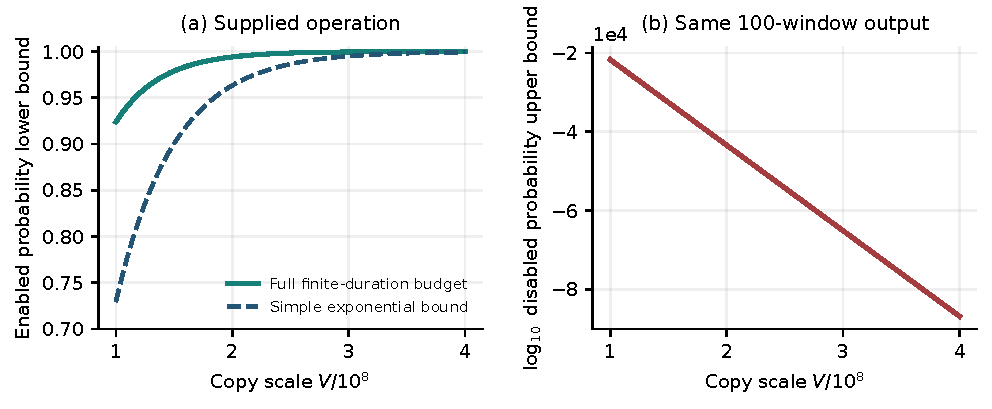
\includegraphics[width=\linewidth]{certificate_bounds.pdf}
\caption{Evaluation of the proved inequalities for the $H=100$ output schedule as the copy scale varies. Left: enabled lower probability from the full budget~\eqref{eq:budget} and from the simplified bound~\eqref{eq:main}. Right: disabled upper bound~\eqref{eq:off} on a logarithmic scale, including resource exits credited as successes. These are numerical evaluations of theorem bounds, not simulations or empirical frequencies.}\label{fig:bounds}
\end{figure}

\subsection{Dimensional conversion and the collected observable}
Let $C_{\mathrm{ref}}$ be a molar reference concentration, $\Omega$ the reactor volume and $d_{\mathrm{ref}}$ the physical dilution rate. Set
\begin{equation}\label{eq:units}
 V=N_AC_{\mathrm{ref}}\Omega,\qquad t=d_{\mathrm{ref}}\,t_{\mathrm{phys}}.
\end{equation}
A first-order dimensionless coefficient $\kappa$ corresponds to the physical rate $\kappa d_{\mathrm{ref}}$, a bimolecular coefficient to $\kappa d_{\mathrm{ref}}/C_{\mathrm{ref}}$; thus $20xu/V$ corresponds to a second-order constant $20d_{\mathrm{ref}}/C_{\mathrm{ref}}$ and $20c_1$ to $20d_{\mathrm{ref}}$. The falling-factorial convention of channel $9$ must be preserved. Driven coefficients are pseudo-first- or pseudo-second-order constants at the chosen reservoir activities, and each feed corresponds to a concentration influx $d_{\mathrm{ref}}C_{\mathrm{ref}}$. Changing $C_{\mathrm{ref}}$ or the dilution rate while holding physical constants fixed changes the dimensionless model. For $C_{\mathrm{ref}}=1\,\mu$M and $d_{\mathrm{ref}}=1$ h$^{-1}$, Table~\ref{tab:example} translates the $V=10^8$, $H=100$ certificate. These are unit translations, not measured productivities or a calibrated protocol. The collected observable is covalent template equivalents carried by $X,C_1,C_2$ and $Z$; dissociation, purification, recovery losses and activity assays would have to be specified before reading it as free active product.

\begin{table}[t]\centering
\caption{Illustrative physical reading of the $V=10^8$, $H=100$ certificate at $C_{\mathrm{ref}}=1\,\mu$M and $d_{\mathrm{ref}}=1$ h$^{-1}$.}\label{tab:example}
\begin{tabular}{lr}\toprule Quantity & Value\\\midrule
Reactor volume & $166.05$ pL\\
Startup allowance & $500$ h\\
Certified post-startup duration & $100$ h\\
Probability of the joint event & $\ge0.9238$\\
Export per completed hour & $\ge20000$ model mass units\\
Covalent $X$ equivalents per hour & $\ge5000$\\
Covalent $X$ equivalents over $100$ h & $\ge5\times10^5$\\
Equivalent product concentration rate & $\ge50$ pM/h\\
Each food-count allowance through $600$ h & $1.2\times10^{11}$\\
Combined gross driving allowance through $600$ h & $7.5\times10^9$\\
Reservoir affinity $(\mu_F-\mu_P)/k_BT$ & $24.88$--$25.29$\\\bottomrule
\end{tabular}
\end{table}

\subsection{Reservoir work}
Under the fixed-potential convention of Remark~\ref{rem:affinity}, the magnitude of the chemical work exchanged through the two service labels up to time $T$ is bounded on $\Son_H$ by
\[
 |\mu_F-\mu_P|\,Q_D(T)\le|\mu_F-\mu_P|\,\frac{VT}8 .
\]
The gross count bounds the absolute sum of the individual exchanges, so reverse events cannot conceal service by net cancellation. Food chemical work, separation, dilution, temperature control, apparatus energy and total entropy production are not priced by this expression, and autonomous finite reservoirs would require a different model; these distinctions follow the open-network accounting of~\citep{rao2018}.

\section{Discussion}\label{sec:discussion}

\paragraph{Why the estimates close.}
Three effective quantities carry the whole argument: resource restoration, a low-count growth and noise margin, and marked export intensity. The competitor leaves the first untouched because it conserves both moieties, and it leaves the second unchanged because its loss falls on free product while the tight phase of the weighted count is bound. Startup is then paid once through a changing exponential test, and the exponential number of observations is paid through one pointwise window bound propagated by induction over the actual continuing distribution; no independence between windows, no restart at entry, and no deterministic approximation is used. The only interaction between the horizon and the volume is the polynomial prefactor of the two leakage terms, which is absorbed into the volume exponent.

\paragraph{The supply side.}
Gross counters on the same law turn the certificate into a ledger: resident inventory stays of order $V$, while food input, washout and driving service over the horizon are of order $VT$. The finite-duration theorem is the practically relevant form, since it lets a reader choose a duration and a confidence and read off the allowances that a fed reactor actually needs; the exponential-horizon statement is its uniform corollary.

\paragraph{The comparison.}
The disabled comparator keeps the same competing cleavage and deletes only templated ligation. Because the comparator receives every resource exit as a possible success and is not asked to establish or reside, the exponential gap between~\eqref{eq:main} and~\eqref{eq:off} is an attribution of the certified output schedule to the templated cycle, for this mechanism and box.

\paragraph{Limits.}
The result gives neither an optimal cleavage tolerance nor an optimal lifetime exponent. The local estimate of Lemma~\ref{lem:local} holds for $\delta\le3/5$, and a fixed-food linearization of the phase dynamics changes sign only around $\delta\approx1.95$ at $80\%$ free food and $\delta\approx3.48$ at $100\%$ free food for $(K,r)=(10,20)$; that boundary is a property of a homogeneous linearization without immigration, not a bifurcation theorem for the fed stochastic reactor, and how much of the gap between the certified interval and that boundary can be recovered while keeping a simple stochastic barrier is an open question. Fixed-volume recurrence and eventual catalyst loss remain compatible with the result. Nothing is claimed for sliding windows, other initial states, a second replicator, or generic random networks, and no experimental calibration is asserted.

\paragraph{Data and code availability.}
The Lean sources, the verification receipt, the interval evaluator and the figure script are described in Appendix~\ref{app:formal}. An independent script re-derives the generator identities of Lemmas~\ref{lem:local} and~\ref{thm:disabled} symbolically and checks every numerical constant of the paper in exact rational arithmetic.

\appendix

\section{Coefficient and bookkeeping checks}\label{app:coeff}
The exact quadratic-rate expression over the twenty channels is
\begin{align*}
 Q_Y={}&(\eps+\delta\eta)\frac{uw}V+(\eps k+\delta)x
 +\frac1{64}\Big(\frac{20xu}V+20c_1\Big)+\Big(\frac{11}{40}\Big)^2\Big(\frac{20c_1w}V+20c_2\Big)\\
 &+\Big(\frac25\Big)^2(20c_2+20kz)+\frac1{25}\Big(rz+\frac{rx(x-1)}V\Big)
 +x+\Big(\frac98\Big)^2c_1+\Big(\frac75\Big)^2c_2+\Big(\frac95\Big)^2z .
\end{align*}
On the low-count corridor use $u/V,w/V\le\frac{11}{10}$, $uw/V^2\le\frac{121}{100}$, $x/V\le\frac1{1000}$, $r\le22$, $k\le\frac18$, $\eps\le10^{-6}$ and $\delta\le\frac1{20}$. The immigration coefficient is at most $\frac{121}{100}\cdot\frac{321}{320}<\frac{25}{16}$, and the coefficients of $x,c_1,c_2,z$ are bounded by
\[
 1+\frac1{20}+\frac{11}{32}+\frac{22}{25000}+\frac1{8\times10^6},\qquad\frac{10374}{3200},\qquad\frac{2669}{400},\qquad\frac{113}{25},
\]
which are below $5,\ \frac{45}8,\ 7,\ 9$ respectively, that is, below $5$ times the weights of $Y$. This proves~\eqref{eq:noise}.

For mass, the washout marks of $M$ are $(2,2,4,6,8,8)$ for $U,W,X,C_1,C_2,Z$ and zero for every other label, and each supported reaction satisfies $\Delta M+\text{washout mass}=2\Delta I_U+2\Delta I_W$; summation gives~\eqref{eq:massbalance}. Each moiety washout mark dominates the export mark divided by four. In the disabled system $\Delta(S+E)/4\le\Delta N_+$ label by label, and only channels $0$ and $19$ increase the right-hand side. These identities account for every material inequality in the text.

\section{Elementary inequalities}\label{app:ineq}
\begin{enumerate}[label=(\roman*)]
\item $e^v\le1+v+\frac35v^2$ for $|v|\le\frac9{50}$: $e^v-1-v=\sum_{m\ge2}v^m/m!\le\frac{v^2}2\sum_{j\ge0}(|v|/3)^j\le\frac{v^2}{2(1-3/50)}=\frac{25}{47}v^2<\frac35v^2$.
\item Bernoulli: $(1+x)^N\ge1+Nx$ for $x\ge0$ and integer $N\ge0$; hence $(1+\frac3{20q})^{10q}\ge\frac52$ and $(1+\frac3{50q})^{10q}\ge\frac85$, and $(5/2)^9=3814.7>2000=(1/20)/(1/40000)$.
\item $e^{-1/2}\le\frac23$, equivalently $e\ge\frac94$; and $e-1<2$.
\item Poisson lower tail: for $J\sim\mathrm{Poisson}(\lambda)$ and $0<\gamma<1$, $\Prob(J<N)\le\gamma^{-N}\E\gamma^J=\exp[N\log(1/\gamma)-(1-\gamma)\lambda]$; with $\lambda=500q$, $N=499q$, $\gamma=\frac{999}{1000}$ the exponent is $q\,[499\log\frac{1000}{999}-\frac12]<-\frac q{500000}$.
\item The startup exponent: $399\cdot\frac{14}{25}\cdot\frac2{25}\cdot\eps-\frac1{2500\cdot40000}=\frac{8047}{312500000000}=\cE$.
\item The window exponent: $\frac1{27000}-\frac1{40000}=\frac{13}{1080000}=\cW$.
\item The disabled slack: $\lambda_{\mathrm{off}}=\frac{38841}{16\times10^{12}}$, $1004\lambda_{\mathrm{off}}<2.44\times10^{-6}$, and $\frac1{21000}-\frac1{25000}=\frac4{525000}>7.6\times10^{-6}$, so the slack in~\eqref{eq:offslack} exceeds $5\times10^{-6}$.
\item For $V\ge10^8$: $e^{(10^{-6}-2\times10^{-8})V}\ge1+0.98\times10^{-6}V\ge99>8$, and $(\cW-2\times10^{-6})V\ge1.0037\times10^{-5}V\ge1003>\frac18$.
\end{enumerate}

\section{Formal evidence and reproducibility}\label{app:formal}
The formal development is in Lean~4~\citep{demoura2021} with Mathlib~\citep{mathlib2020}, toolchain \lean{leanprover/lean4:v4.30.0} and a frozen manifest. The verification bridge treats warnings as errors and accepts no \lean{sorry}; a successful receipt has exit code zero and empty compiler output. The endpoint that packages the results of this paper is
\begin{center}
\lean{RandomViability.Binding.competition_publication_probability}
\end{center}
in \lean{proofs/RandomViability/BindingCompetitionPublication.lean}. Its statement, transcribed, is: for every natural $V\ge10^8$, every natural number $m$ of complete windows and nonnegative real final fraction $s$ with $m+s\le e^{V/10^6}$, and every parameter triple in the box, the expectation of the indicator of the joint good event (window history, pass bit, and the three duration-specific supply budgets) under the joint finite law is at least $1-2\exp(-2V/10^8)$. It is obtained from the finite-duration theorem \lean{competition_timed_supplied_probability}, which bounds the same expectation below by $1-\mathcal B(V,m+s)$ for every $V>0$, and from the scalar bound \lean{competition_timed_error_bound}. Table~\ref{tab:formal} maps the steps of this paper to the modules of the development; all modules are under \lean{proofs/RandomViability/} and carry the prefix \lean{BindingCompetition}.

\begin{table}[ht]\centering\small
\caption{Critical-path formal source map (namespace \texttt{RandomViability.Binding}).}\label{tab:formal}
\begin{tabular}{>{\raggedright\arraybackslash}p{0.36\textwidth}>{\raggedright\arraybackslash}p{0.56\textwidth}}\toprule
Step in this paper & Module suffixes and principal declarations\\\midrule
Source, moieties, marks (Section~\ref{sec:model}) & Source, Bookkeeping, ContractModel: \lean{competition_rate_support}, \lean{competition_covalent_balance}, \lean{competition_total_rate_bound}\\
Lemma~\ref{lem:resources} & Resources, ResourceTails: \lean{competition_resource_probability}\\
Lemma~\ref{lem:local} & Drift, Exponential: \lean{competition_corridor_growth}, \lean{competition_variance_envelope}, \lean{competition_corridor_exponential}\\
Lemma~\ref{lem:entryreturn}, entry & EntryKernel, EntrySchedule, EntryProbability, TrackedEntry, EntryLaw: \lean{competition_entry_hundred_clock_transfer}, \lean{competition_entry_deadline}\\
Lemma~\ref{lem:entryreturn}, return & Return, TrackedReturn: \lean{competition_tracked_return_probability}\\
Lemma~\ref{lem:windows} & WindowModel, WindowProbability, WindowRounded, WindowHistory, AllWindows: \lean{competition_unit_window_probability}, \lean{competition_all_windows_probability}\\
Composition over the schedule & MonitorFoster, HorizonWindows, HorizonComposition, FinalFraction, ContractModel\\
Lemma~\ref{lem:supplies} & GrossCounters, CounterTilt, JointModel, JointCounterBounds, JointSupplyTails, CounterHistory: \lean{competition_cap_preserves_sum_failure}\\
Theorem~\ref{thm:main}, \eqref{eq:finite} & Timed: \lean{competition_timed_supplied_probability}\\
Theorem~\ref{thm:main}, \eqref{eq:main} & SuppliedOperating, ErrorBudget, Sizing, Publication: \lean{competition_supplied_operating_probability}, \lean{competition_timed_error_bound}, \lean{competition_publication_probability}\\
Theorem~\ref{thm:disabled} & DisabledSource, DisabledProbability, Comparison, TimedComparison: \lean{competition_disabled_comparison}, \lean{competition_timed_disabled_comparison}\\
Corollaries~\ref{cor:output}, \ref{cor:cost} & Throughput, Scaling, Consequences: \lean{competition_arbitrary_interval}, \lean{competition_timed_expected_guarantee}, \lean{competition_service_ratio}, \lean{competition_recovery_ratio}, \lean{competition_replenishment}\\
Sizing rule~\eqref{eq:sizing} & Sizing: \lean{competition_duration_sizing}, \lean{competition_confidence_sizing}\\
\bottomrule
\end{tabular}
\end{table}

The recorded strict verification of the publication endpoint compiled with empty compiler output in $130.6$~s together with $86$ authenticated dependency modules; the SHA-256 of the endpoint source is
\begin{center}\footnotesize\ttfamily
510f465f79a63e99f668824cc990bf72165d089b650c5381afb17d0f4646e4be .
\end{center}
Within the development, verification is reproduced from the repository root by
\begin{quote}\footnotesize\ttfamily
python scripts/verify\_proof.py \textbackslash\\
\hspace*{2em}proofs/RandomViability/BindingCompetitionPublication.lean \textbackslash\\
\hspace*{2em}--timeout 600 \textbackslash\\
\hspace*{2em}--declaration RandomViability.Binding.competition\_publication\_probability
\end{quote}
which pins the working directory and toolchain. The proofs are symbolic over the parameter box and over all $V$, $m$ and $s$; no enumeration of states, windows or counters, no floating-point evaluation and no simulation enters as evidence.

\paragraph{Formal scope.}
Lean verifies the finite marked laws, the source estimates of Lemmas~\ref{lem:resources}--\ref{lem:supplies}, the projections and saturation lemmas of Section~\ref{sec:formal}, the induction over windows, the union bounds, the scalar inequalities behind~\eqref{eq:main}, the disabled comparison, and the interval geometry and ratio inequalities of Section~\ref{sec:consequences}. The expectation declaration bounds the finite guaranteed-output indicator; its comparison with the uncapped literal path export in~\eqref{eq:expectation}, the nonexplosion and identification arguments of Section~\ref{sec:formal}, the channel-history reading of the mass balance, and Remark~\ref{rem:startup} are conventional. The reservoir affinity~\eqref{eq:affinity} and the dimensional translation of Section~\ref{sec:example} are interpretations. The interval evaluator and the figures are numerical evaluations of proved formulas and are not kernel evidence.

\bibliographystyle{plainnat}
\bibliography{refs}

\end{document}
